\documentclass[11pt]{standalone}

\usepackage{tikz}
\usetikzlibrary{positioning, arrows.meta, shapes.misc}

\begin{document}
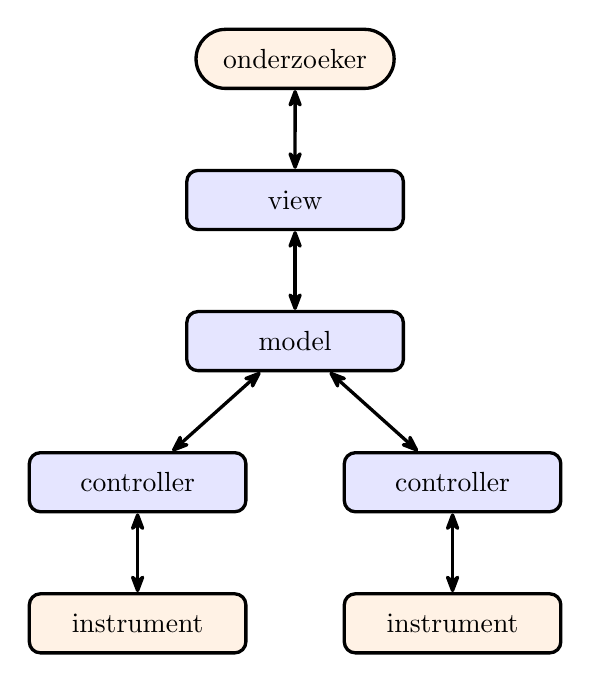
\begin{tikzpicture}[draw, very thick, every node/.style={draw, rounded corners, minimum width=2.75cm, minimum height=.75cm, node distance=1cm}, >={Stealth[round]}]
    \node[fill=orange!10, sharp corners, rounded rectangle] (user) {onderzoeker};
    \node[fill=blue!10] (view) [below=of user] {view};
    \node[fill=blue!10] (model) [below=of view] {model};
    \node[fill=blue!10] (controller1) [below=of model,xshift=-2cm] {controller};
    \node[fill=blue!10] (controller2) [below=of model,xshift=2cm] {controller};
    % \path (controller1) -- (controller2) node[midway,scale=2,lightgray,draw=none] {$\ldots$};
    \node[fill=orange!10] (dev1) [below=of controller1] {instrument};
    \node[fill=orange!10] (dev2) [below=of controller2] {instrument};
    % \path (dev1) -- (dev2) node[midway,scale=2,lightgray,draw=none] {$\ldots$};

    \draw[<->] (user) -- (view);
    \draw[<->] (view) -- (model);
    \draw[<->] (model) -- (controller1);
    \draw[<->] (model) -- (controller2);
    \draw[<->] (controller1) -- (dev1);
    \draw[<->] (controller2) -- (dev2);
\end{tikzpicture}
\end{document}